\documentclass[11pt,twoside,draft,final]{article}
\usepackage{amsmath,amsfonts,amssymb,amsthm,indentfirst,enumerate,textcomp}
\usepackage[utf8]{inputenc}
\usepackage{tikz}

\begin{document}

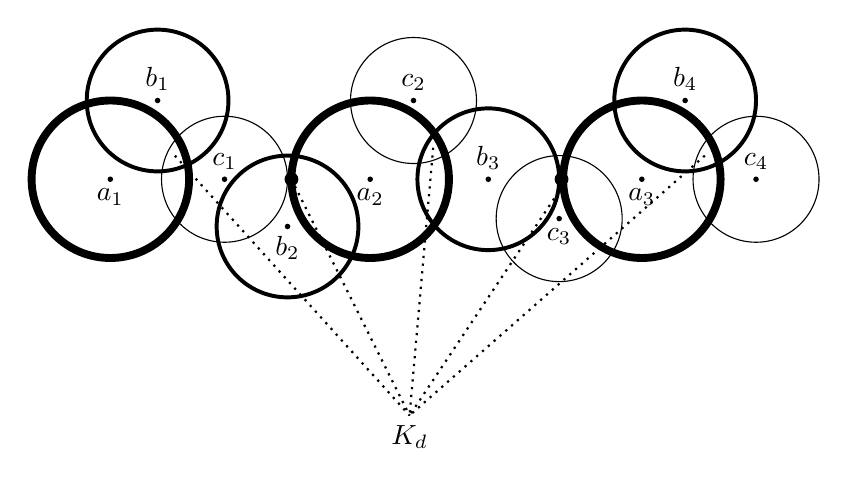
\begin{tikzpicture}
		\draw[line width=1mm] (-3.3,0) circle(1);
		\fill[fill=black](-3.3,0) circle (1pt) node[below] {$a_1$};
		
		\draw[line width=0.5mm] (-2.7,1) circle(0.9);
		\fill[fill=black](-2.7,1) circle (1pt) node[above] {$b_1$};
		
		\draw[thin] (-1.85,0) circle(0.8);
		\fill[fill=black](-1.85,0) circle (1pt) node[above] {$c_1$};
		
		\draw[line width=1mm] (0,0) circle(1);
		\fill[fill=black](0,0) circle (1pt) node[below] {$a_2$};		
		
		\draw[line width=0.5mm] (-1.05,-0.6) circle(0.9);
		\fill[fill=black](-1.05,-0.6) circle (1pt) node[below] {$b_2$};
		
		\draw[line width=0.5mm] (1.5,0) circle(0.9);
		\fill[fill=black](1.5,0) circle (1pt) node[above] {$b_3$};

		\draw[thin] (0.55,1) circle(0.8);
		\fill[fill=black](0.55,1) circle (1pt) node[above] {$c_2$};
		
		\draw[line width=1mm] (3.45,0) circle(1);
		\fill[fill=black](3.45,0) circle (1pt) node[below] {$a_3$};
		
		\draw[thin] (2.4,-0.5) circle(0.8);
		\fill[fill=black](2.4,-0.5) circle (1pt) node[below] {$c_3$};
		
		\draw[thin] (4.9,0) circle(0.8);
		\fill[fill=black](4.9,0) circle (1pt) node[above] {$c_4$};
		
		\draw[line width=0.5mm] (4,1) circle(0.9);
		\fill[fill=black](4,1) circle (1pt) node[above] {$b_4$};		
						
		
		\fill[fill=black](2.43,0) circle (2.5pt) node[below] {};
		\fill[fill=black](-1,0) circle (2.5pt) node[below] {};
		
		\draw[thick, dotted] (4.25,0.3) to (0.5,-3) node[below] {$K_d$};
		\draw[thick, dotted] (2.5,0) to (0.5,-3) node[below] {};
		\draw[thick, dotted] (0.8,0.4) to (0.5,-3) node[below] {};
		\draw[thick, dotted] (-1,0) to (0.5,-3) node[below] {};
		\draw[thick, dotted] (-2.48,0.3) to (0.5,-3) node[below] {};
		\end{tikzpicture}

\end{document}